\documentclass[]{article}
\usepackage{lmodern}
\usepackage{amssymb,amsmath}
\usepackage{ifxetex,ifluatex}
\usepackage{fixltx2e} % provides \textsubscript
\ifnum 0\ifxetex 1\fi\ifluatex 1\fi=0 % if pdftex
  \usepackage[T1]{fontenc}
  \usepackage[utf8]{inputenc}
\else % if luatex or xelatex
  \ifxetex
    \usepackage{mathspec}
  \else
    \usepackage{fontspec}
  \fi
  \defaultfontfeatures{Ligatures=TeX,Scale=MatchLowercase}
\fi
% use upquote if available, for straight quotes in verbatim environments
\IfFileExists{upquote.sty}{\usepackage{upquote}}{}
% use microtype if available
\IfFileExists{microtype.sty}{%
\usepackage{microtype}
\UseMicrotypeSet[protrusion]{basicmath} % disable protrusion for tt fonts
}{}
\usepackage[margin=1in]{geometry}
\usepackage{hyperref}
\hypersetup{unicode=true,
            pdfborder={0 0 0},
            breaklinks=true}
\urlstyle{same}  % don't use monospace font for urls
\usepackage{color}
\usepackage{fancyvrb}
\newcommand{\VerbBar}{|}
\newcommand{\VERB}{\Verb[commandchars=\\\{\}]}
\DefineVerbatimEnvironment{Highlighting}{Verbatim}{commandchars=\\\{\}}
% Add ',fontsize=\small' for more characters per line
\newenvironment{Shaded}{}{}
\newcommand{\KeywordTok}[1]{\textcolor[rgb]{0.00,0.44,0.13}{\textbf{{#1}}}}
\newcommand{\DataTypeTok}[1]{\textcolor[rgb]{0.56,0.13,0.00}{{#1}}}
\newcommand{\DecValTok}[1]{\textcolor[rgb]{0.25,0.63,0.44}{{#1}}}
\newcommand{\BaseNTok}[1]{\textcolor[rgb]{0.25,0.63,0.44}{{#1}}}
\newcommand{\FloatTok}[1]{\textcolor[rgb]{0.25,0.63,0.44}{{#1}}}
\newcommand{\ConstantTok}[1]{\textcolor[rgb]{0.53,0.00,0.00}{{#1}}}
\newcommand{\CharTok}[1]{\textcolor[rgb]{0.25,0.44,0.63}{{#1}}}
\newcommand{\SpecialCharTok}[1]{\textcolor[rgb]{0.25,0.44,0.63}{{#1}}}
\newcommand{\StringTok}[1]{\textcolor[rgb]{0.25,0.44,0.63}{{#1}}}
\newcommand{\VerbatimStringTok}[1]{\textcolor[rgb]{0.25,0.44,0.63}{{#1}}}
\newcommand{\SpecialStringTok}[1]{\textcolor[rgb]{0.73,0.40,0.53}{{#1}}}
\newcommand{\ImportTok}[1]{{#1}}
\newcommand{\CommentTok}[1]{\textcolor[rgb]{0.38,0.63,0.69}{\textit{{#1}}}}
\newcommand{\DocumentationTok}[1]{\textcolor[rgb]{0.73,0.13,0.13}{\textit{{#1}}}}
\newcommand{\AnnotationTok}[1]{\textcolor[rgb]{0.38,0.63,0.69}{\textbf{\textit{{#1}}}}}
\newcommand{\CommentVarTok}[1]{\textcolor[rgb]{0.38,0.63,0.69}{\textbf{\textit{{#1}}}}}
\newcommand{\OtherTok}[1]{\textcolor[rgb]{0.00,0.44,0.13}{{#1}}}
\newcommand{\FunctionTok}[1]{\textcolor[rgb]{0.02,0.16,0.49}{{#1}}}
\newcommand{\VariableTok}[1]{\textcolor[rgb]{0.10,0.09,0.49}{{#1}}}
\newcommand{\ControlFlowTok}[1]{\textcolor[rgb]{0.00,0.44,0.13}{\textbf{{#1}}}}
\newcommand{\OperatorTok}[1]{\textcolor[rgb]{0.40,0.40,0.40}{{#1}}}
\newcommand{\BuiltInTok}[1]{{#1}}
\newcommand{\ExtensionTok}[1]{{#1}}
\newcommand{\PreprocessorTok}[1]{\textcolor[rgb]{0.74,0.48,0.00}{{#1}}}
\newcommand{\AttributeTok}[1]{\textcolor[rgb]{0.49,0.56,0.16}{{#1}}}
\newcommand{\RegionMarkerTok}[1]{{#1}}
\newcommand{\InformationTok}[1]{\textcolor[rgb]{0.38,0.63,0.69}{\textbf{\textit{{#1}}}}}
\newcommand{\WarningTok}[1]{\textcolor[rgb]{0.38,0.63,0.69}{\textbf{\textit{{#1}}}}}
\newcommand{\AlertTok}[1]{\textcolor[rgb]{1.00,0.00,0.00}{\textbf{{#1}}}}
\newcommand{\ErrorTok}[1]{\textcolor[rgb]{1.00,0.00,0.00}{\textbf{{#1}}}}
\newcommand{\NormalTok}[1]{{#1}}
\usepackage{graphicx,grffile}
\makeatletter
\def\maxwidth{\ifdim\Gin@nat@width>\linewidth\linewidth\else\Gin@nat@width\fi}
\def\maxheight{\ifdim\Gin@nat@height>\textheight\textheight\else\Gin@nat@height\fi}
\makeatother
% Scale images if necessary, so that they will not overflow the page
% margins by default, and it is still possible to overwrite the defaults
% using explicit options in \includegraphics[width, height, ...]{}
\setkeys{Gin}{width=\maxwidth,height=\maxheight,keepaspectratio}
\IfFileExists{parskip.sty}{%
\usepackage{parskip}
}{% else
\setlength{\parindent}{0pt}
\setlength{\parskip}{6pt plus 2pt minus 1pt}
}
\setlength{\emergencystretch}{3em}  % prevent overfull lines
\providecommand{\tightlist}{%
  \setlength{\itemsep}{0pt}\setlength{\parskip}{0pt}}
\setcounter{secnumdepth}{0}
% Redefines (sub)paragraphs to behave more like sections
\ifx\paragraph\undefined\else
\let\oldparagraph\paragraph
\renewcommand{\paragraph}[1]{\oldparagraph{#1}\mbox{}}
\fi
\ifx\subparagraph\undefined\else
\let\oldsubparagraph\subparagraph
\renewcommand{\subparagraph}[1]{\oldsubparagraph{#1}\mbox{}}
\fi

%%% Use protect on footnotes to avoid problems with footnotes in titles
\let\rmarkdownfootnote\footnote%
\def\footnote{\protect\rmarkdownfootnote}

%%% Change title format to be more compact
\usepackage{titling}

% Create subtitle command for use in maketitle
\newcommand{\subtitle}[1]{
  \posttitle{
    \begin{center}\large#1\end{center}
    }
}

\setlength{\droptitle}{-2em}

  \title{}
    \pretitle{\vspace{\droptitle}}
  \posttitle{}
    \author{}
    \preauthor{}\postauthor{}
    \date{}
    \predate{}\postdate{}
  

\begin{document}

\section{Rapport du travail effectué sur les TP1 et 2 d'algorithmique
générale}\label{rapport-du-travail-effectue-sur-les-tp1-et-2-dalgorithmique-generale}

J'ai choisi pour ce projet de créer une forge pour pouvoir travailler
chez moi et à l'école. De plus vu la taille du programme, j'ai choisis
de programmer de façon modulaire afin que les temps de compilation
soient réduits. J'ai donc écris un \texttt{MakeFile} que vous trouverez
en annexe.

\subsection{Partie A : Préliminaire}\label{partie-a-preliminaire}

J'ai choisi comme structure d'implémenter un graphe sous ses trois
formes : une matrice d'adjacence, une liste pi et alpha et une liste de
successeurs.

\begin{Shaded}
\begin{Highlighting}[]
\KeywordTok{typedef} \KeywordTok{struct} \NormalTok{Graphe\{}
    \DataTypeTok{int} \NormalTok{nb_aretes;}
    \DataTypeTok{int} \NormalTok{nb_sommets;}
    \DataTypeTok{int} \NormalTok{oriente;}
    \DataTypeTok{int} \NormalTok{*pi;}
    \DataTypeTok{int} \NormalTok{*alpha;}
    \DataTypeTok{int} \NormalTok{**liste_adjacence;}
    \DataTypeTok{int} \NormalTok{**liste_successeurs;}
\NormalTok{\}Graphe;}
\end{Highlighting}
\end{Shaded}

La première partie du TP était assez simple à implémenter, jusqu'au dfs,
qui lui m'a pris beaucoup de temps. De plus la question sur la connexité
a du être retravaillée pour répondre aux attentes du sujet. La
compléxité de chacune des fonctions sera détaillée dans la dernière
partie.

\subsubsection{Question 1 :}\label{question-1}

La fonction
\texttt{Graphe*\ create\_from\_file(char\ nom\_de\_fichier{[}{]})}
permet d'implémenter ma structure graphique à partir d'un graphe décrit
en fichier texte. Cette fonction implémente tout d'abord la matrice
d'adjacence, qui est plus facile à manipuler. Ensuite la fonctiuon
\texttt{void\ initialize\_all(Graphe\ *graph)} initialise les valeurs de
pi, alpha et de la matrice des successeurs. Lorsque l'on execute le
main, on peut entrer à l'aide d'un scanf, le nom du graphe que l'on
souhaite étudier par exemple \texttt{digraph-1.txt}. Une fois ses
représentations initialisées, on peut travailler avec le graphe.

\subsubsection{Question 2 :}\label{question-2}

Afin de répondre à cette question, j'ai utilisé la matrice d'adjacence,
qui me paraissait plus simple à utiliser. A partir de celle-ci, je crée
un fichier .dot en utilisant la syntaxe universelle dot. Je pourrais
pour améliorer l'efficacité de cette fonction en utilisant la liste
d'adjacence, mais je n'ai pas eu le temps de revenir dessus.

\subsubsection{Question 3 :}\label{question-3}

J'ai écrit 5 fonctions de dfs qui ont chacune une utilité particulière.
Cependant la forme des ces 5 fonctions est toujours la même : la
fonction
\texttt{void\ dfs(Graphe\ *graphe,int\ sommet\_depart\ ,liste\_ordre\ **ordre\_par\_sommet,\ int\ **sommet\_marque\_dugraphe)}
que j'ai baptisé ``le gros dfs'' utilise la fonction
\texttt{void\ dfss(Graphe\ *graphe,int\ sommet,\ int\ *sommet\_marque,\ liste\_ordre\ *ordre)}
que j'ai surnommée ``le petit dfs''. Le petit dfs prend en entrée un
sommet, dont il va parcourir le premier successeur en profondeur pour
ensuite parcourir ses autres successeurs aussi en profondeur. Pour
chaque sommet parcouru, le sommet est marqué et le sommet est aussi
ajouté à l'ordre de parcours du dfs qui est stocké sous la forme d'une
liste chainée. De plus, l'un des dfs permet de créer l'arbre dfs, ou
l'arbre de parcour suprimant les arretes non utilisées par le parcour.
Sur les 5 dfs codé, 4 utilisent la matrice pi et alpha, qui permettent
d'avoir la meilleure implémentation possible. La forme des tableaux
d'ordre renvoyés par les dfs s'affiche sous la forme :

\texttt{{[}1-\textgreater{}2-\textgreater{}3-\textgreater{}4{]}\ \ \ \ \ {[}5-\textgreater{}6-\textgreater{}7{]}}

L'un des petits dfs utilise la matrice d'adjacence qui est nécessaire
pour trouver l'orientation forte d'un graphe non orienté.

\subsubsection{Question 4 :}\label{question-4}

Afin de teste si un graphe est connexe, j'ai juste à utiliser la
fonction de dfs que j'ai implémentée précédement. Si le graphe donné en
entrée est orienté, je dois le ``dés-orienter'' le rendre non orienté
car l'ordre n'est pas important pour la connexité. Ensuite il ne me
reste plus qu'à lancer un dfs et si le tableau des ordre de parcour
renvoyé par mon dfs contient deux ordre de parcours, cela veut dire que
à partir d'un des sommets, le grand dfs ne parvient pas à marquer un
autres des sommets et doit donc relancer le petit dfs sur celui ci. Cela
implique qu'un sommet est donc isolé et que la graphe n'est donc pas
connexe. La condition de connexité est donc très simple à vérifier.

\subsubsection{Question 5 :}\label{question-5}

L'inversion du graphe orienté se fait en utilisant la matrice
d'adjacence - c'est la fonction la plus couteuse en terme de mémoire -
et la fonction \texttt{void\ initialize\_all(Graphe\ *graph)} pour
ensuite mettre à jour le graph obtenu.

\subsection{Partie B : Composantes fortement
connexes}\label{partie-b-composantes-fortement-connexes}

Cette partie du TD à été la plus longue et laborieuse : c'est nottement
pour cette partie que j'ai du écrire plusieurs dfs.

\subsubsection{Question 1 \& 3:}\label{question-1-3}

Pour déterminer les composantes fortement connexes j'ai utilisé
l'algorithme de kosaraju, qui utilise un premier dfs (pu l'on ajoute le
sommet parcouru qu'une fois qu'on a parcouru tous ses successeurs) puis
un deuxième dfs appliqué à l'inverse du graphe en utilisant l'ordre de
parcour inverse obtenue lors du premier dfs. Le tableau d'ordre retourné
par ce deuxième dfs contient les composantes fortement connexes de ce
graphe. A partir de ce tableau, je crée un deuxième graphe, contenant en
sous graphe les composantes fortement connexes. J'ai aussi utilisé
l'hypothèse qu'une composante toute seule est fortement connexe. Voici
le graphe rendu par mon algorythme, appliqué sur le digraph-1.

\begin{figure}[htbp]
\centering

\includegraphics{./Images/polytech.jpg}
\caption{Image}
\end{figure}

\subsubsection{Question 2 :}\label{question-2-1}

La complexité de cette algorithme est : \texttt{O(N²)} à cause de
l'invertion. Sans cette étape d'invertion, la complexité est linéaire.

\subsubsection{Question 3 :}\label{question-3-1}

'cf question 1 pour la premi'ai du écrire une nouvelle fonction appelée
\texttt{void\ create\_dot2(Graphe\ *graphe,\ char\ nom\_de\_fichier{[}{]},liste\_ordre\ **composantes,\ int\ nbc);}
qui prend donc en entrées les composantes fortement connexe et re-écrit
le graph, en utilisant une petite astuce: toutes les sommets des
composantes fortement connexes sont simplement placées dans un sous
graphe, sans aucune liaisons. Ci après le fichier.dot et .ps rendu par
l'algorithme après exécution sur le digraph-1.

\begin{Shaded}
\begin{Highlighting}[]
\NormalTok{digraph premier_graph \{}
    \NormalTok{subgraph cluster_0 \{}
        \DecValTok{3}\NormalTok{;}
        \DecValTok{1}\NormalTok{;}
        \DecValTok{2}\NormalTok{;}
        \DecValTok{4}\NormalTok{;}
 
    \NormalTok{\}}
    \NormalTok{subgraph cluster_1 \{}
        \DecValTok{8}\NormalTok{;}
    \NormalTok{\}   subgraph cluster_2 \{}
        \DecValTok{10}\NormalTok{;}
    \NormalTok{\}   subgraph cluster_3 \{}
        \DecValTok{9}\NormalTok{;}
    \NormalTok{\}   subgraph cluster_5 \{}
        \DecValTok{5}\NormalTok{;}
        \DecValTok{7}\NormalTok{;}
        \DecValTok{6}\NormalTok{;}
 
    \NormalTok{\}}
\DecValTok{1} \NormalTok{-> }\DecValTok{3} \NormalTok{;}
\DecValTok{2} \NormalTok{-> }\DecValTok{1} \NormalTok{;}
\DecValTok{2} \NormalTok{-> }\DecValTok{3} \NormalTok{;}
\DecValTok{3} \NormalTok{-> }\DecValTok{4} \NormalTok{;}
\DecValTok{3} \NormalTok{-> }\DecValTok{8} \NormalTok{;}
\DecValTok{4} \NormalTok{-> }\DecValTok{2} \NormalTok{;}
\DecValTok{4} \NormalTok{-> }\DecValTok{5} \NormalTok{;}
\DecValTok{4} \NormalTok{-> }\DecValTok{6} \NormalTok{;}
\DecValTok{5} \NormalTok{-> }\DecValTok{6} \NormalTok{;}
\DecValTok{6} \NormalTok{-> }\DecValTok{7} \NormalTok{;}
\DecValTok{7} \NormalTok{-> }\DecValTok{5} \NormalTok{;}
\DecValTok{8} \NormalTok{-> }\DecValTok{9} \NormalTok{;}
\DecValTok{8} \NormalTok{-> }\DecValTok{10} \NormalTok{;}
\DecValTok{9} \NormalTok{-> }\DecValTok{10} \NormalTok{;}
\NormalTok{\}}
\end{Highlighting}
\end{Shaded}

\begin{figure}[htbp]
\centering
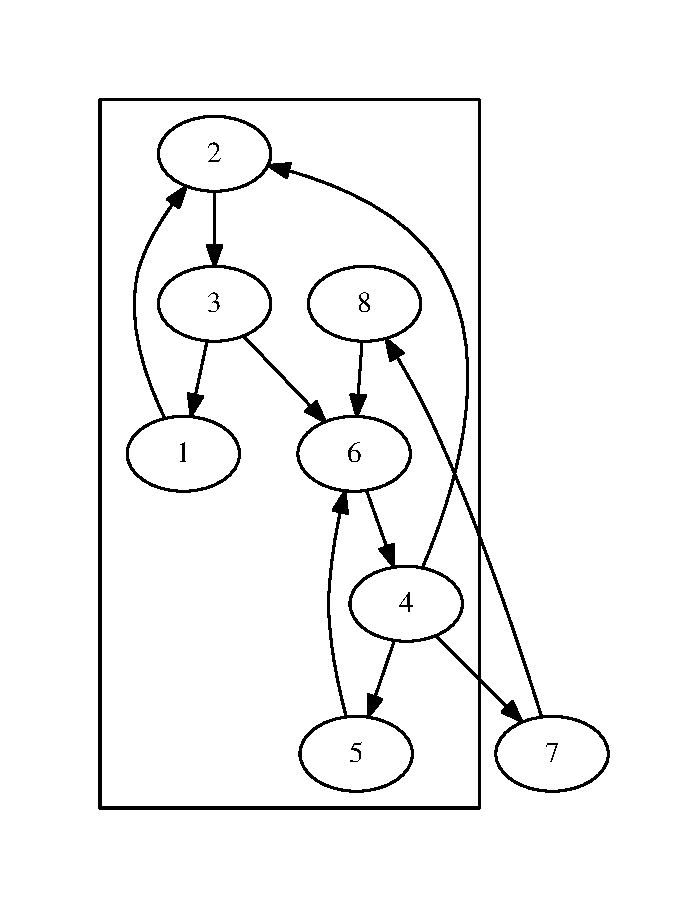
\includegraphics{./Images/orifortecfc.pdf}
\caption{Image}
\end{figure}

\subsection{Partie C : Orientation forte d'un
graphe}\label{partie-c-orientation-forte-dun-graphe}

Partie assez facile seulement, la dernière question n'est pas
implémentée de la bonne manière.

\subsubsection{Question 1 :}\label{question-1-1}

La procédure utilise la matrice d'adjacence pour supprimer chacunes des
arretes. Ensuite on vérifie si le graphe donné en entreé est encore
connexe ou pas. La complexité de cette fonction est polynomiale :
\(O(N²)\) . Je n'ai pas trouvé de méthode linéaire permettant la
suppression d'une arrete.

\subsubsection{Question 2 :}\label{question-2-2}

A faire

\subsubsection{Question 3 :}\label{question-3-2}

On doit tout d'abord vérifier que le graphe ne possède pas de ponts,
ensuite on effectue une procédure que j'ai trouvé sur Wikipédia, qui
conciste à effectuer un dfs à partir d'un sommet, pour ensuite orienter
toutes les arretes des sommets parcouruts dans le sens du dfs, et toutes
les arretes restantes vers la racine, donc dans l'autre sens. La
compléxité de cette algorithme est :

\subsubsection{Question 4:}\label{question-4-1}

Vous trouverez ci joint une orientation du graphique K proposé dans
l'énoncé ainsi qu'une autre orientation du graphique H.

\begin{figure}[htbp]
\centering
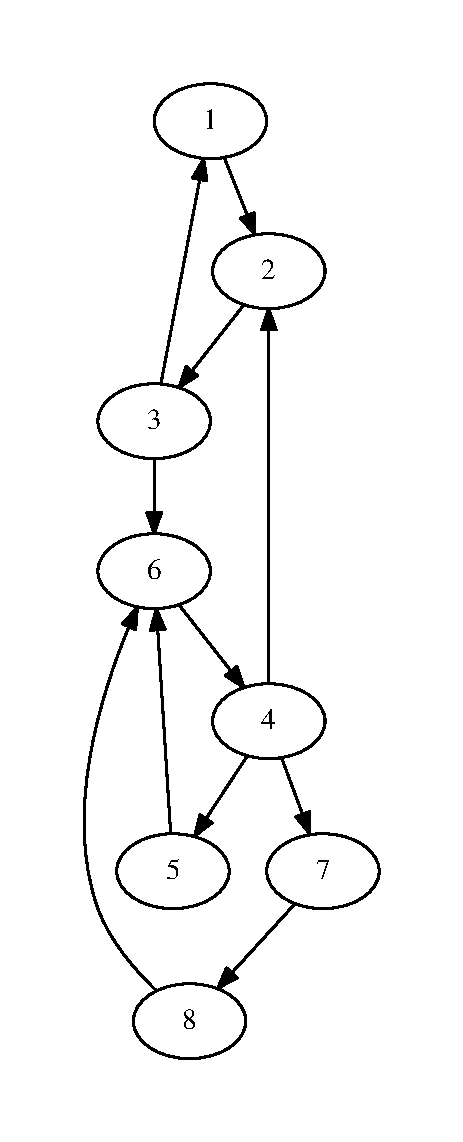
\includegraphics{./Images/oriforte.pdf}
\caption{Image}
\end{figure}

\section{References}\label{references}

\section{Annexes:}\label{annexes}

\subsection{Makefile :}\label{makefile}

\begin{Shaded}
\begin{Highlighting}[]
\KeywordTok{CC} \NormalTok{= gcc}
\KeywordTok{LDFLAGS} \NormalTok{= -Wall -g}
\KeywordTok{LIB} \NormalTok{= }\OtherTok{$(}\KeywordTok{wildcard} \NormalTok{*.c}\OtherTok{)}
\KeywordTok{OBJ} \NormalTok{= }\OtherTok{$(}\KeywordTok{LIB}\NormalTok{:.c=.o}\OtherTok{)}
\KeywordTok{all}\NormalTok{: main}
\KeywordTok{.depend}\NormalTok{:}
    \OtherTok{$(}\KeywordTok{CC}\OtherTok{)} \KeywordTok{-MM} \OtherTok{$(}\KeywordTok{LIB}\OtherTok{)}
\KeywordTok{%.o}\NormalTok{:%.c}
    \OtherTok{$\{CC\}} \OtherTok{$\{LDFLAGS\}} \NormalTok{$^ }\KeywordTok{-c} \NormalTok{-o }\OtherTok{$@}
\KeywordTok{libfonctions.a}\NormalTok{: }\OtherTok{$\{OBJ\}}
    \KeywordTok{ar} \NormalTok{-cru  }\OtherTok{$@} \NormalTok{$^}
    \KeywordTok{ranlib} \OtherTok{$@}
\KeywordTok{main}\NormalTok{: }\OtherTok{$\{OBJ\}} \NormalTok{libfonctions.a}
    \OtherTok{$(}\KeywordTok{CC}\OtherTok{)} \OtherTok{$(}\KeywordTok{OBJ}\OtherTok{)} \KeywordTok{-o} \OtherTok{$@}
    \KeywordTok{valgrind} \NormalTok{--leak-check=full --track-origins=yes ./main}
    \KeywordTok{dot} \NormalTok{-Tpdf digraph-1-strong_orientationfc.dot -o ./Images/orifortecfc.pdf}
    \KeywordTok{dot} \NormalTok{-Tpdf digraph-1-strong_orientation.dot  -o ./Images/oriforte.pdf}
    \KeywordTok{dot} \NormalTok{-Tpdf digraph-1-predfs.dot  -o ./Images/predf.pdf}
    \KeywordTok{dot} \NormalTok{-Tpdf digraph-1-postdfs.dot  -o ./Images/postdfs.pdf}
    \KeywordTok{dot} \NormalTok{-Tpdf digraph-1-compoaprèscfc.dot -o ./Images/compoaprèscfc.pdf}

\KeywordTok{clean}\NormalTok{:}
    \KeywordTok{rm} \NormalTok{-rf *.o main libfonctions.a *.dot *.ps}
\KeywordTok{.PHONY}\NormalTok{: clean}
\end{Highlighting}
\end{Shaded}


\end{document}
